
%
%  $Description: Author guidelines and sample document in LaTeX 2.09$ 
%
%  $Author: ienne $
%  $Date: 1995/09/15 15:20:59 $
%  $Revision: 1.4 $
%

\documentclass[times, 10pt,twocolumn]{article} 
\usepackage{latex8}
\usepackage{times}
\usepackage{graphicx}
\usepackage{amsmath}
\usepackage{verbatim}
\usepackage{subfigure}

%\documentstyle[times,art10,twocolumn,latex8]{article}

%------------------------------------------------------------------------- 
% take the % away on next line to produce the final camera-ready version 
\pagestyle{empty}

%------------------------------------------------------------------------- 
\begin{document}

\title{A Weighted Congruence Measure}

\author{Irwin Kwan, Adrian Schr{\"o}ter, and Daniela Damian\\
Software Engineering Global interAction Lab, Department of Computer Science\\
University of Victoria, Canada\\ 
\{irwink,schadr,danielad\}@cs.uvic.ca\\
}

\maketitle
\thispagestyle{empty}

\begin{abstract}
Socio-technical congruence is an intuitive way to compare required coordination effort within a software development project with the actual ongoing coordination.
The current model of congruence is limited because it builds on top of some simplifying assumptions.
These assumptions, such as placing equal importance of coordination needs, often fail to reflect the actual nature of a project.
We propose a model that derives actual coordination needs from fine grained task interdependencies and task assignments.
This enables us to compare those needs with the real ongoing coordination other than just dichotomized measurements.
\end{abstract}



%------------------------------------------------------------------------- 
\Section{Introduction}
Building good software requires coordination among developers and within teams. 
People who work on related software components should also coordinate their efforts with each other. 
Socio-technical congruence is a measurement that computes the alignment between the social coordination and with the technical dependencies as imposed by the project tasks ~\cite{cataldo2006:coordination_reqs}. 
The result is a ratio of how well the social connections among people match the technical dependencies among people.

The measurement of socio-technical congruence allows observers to study project with a ``fine-grained'' perspective of dependent tasks.
A manager can use this measurement to view the alignment of his teams' coordination with the technical dependencies. 
%This intuitive approach makes up congruence.
Unfortunately, the measure of congruence presented by Cataldo, et al~\cite{cataldo2006:coordination_reqs} uses dichotomized values for its relationships between people, resulting in a coarse interaction model.

We propose an improvement to the original congruence calculation.
The improvement enables us to model the connections more fine grained by applying weights to each relationship.
Weights provides a measure of strength between people and tasks, interdependent tasks, and between people.
Thus, we can reflect organizational social and technical interactions more precisely.
Hence, our resulting congruence measurement is a more precise measure of congruence than a measurement that uses dichotomized relationship strengths.
% We believe that modelling congruence using weighted edges provides us a more accurate reflection of the organization, allowing us to investigate the interactions between individuals in more detail.

This refinement is necessary because the current way of modelling congruence is based on some implicit assumptions.
Two of those assumptions are that every dependency is equally important, and that any coordination is good enough to satisfy a coordination need.
Stepping away from those assumptions is important in order to more accurately model coordination, and to apply congruence to a larger set of projects.


%Stepping away from those assumptions is important to support more vital coordination needs and to ensure that the coordination is not only present, but also sufficient.


In the remainder of this work, we start with describing the related work (Section~\ref{sec:relwork}), followed by the description of our measurement (Section~\ref{sec:measure}).
After discussing the benefits of this new measurement in Section~\ref{sec:benefit}, we end with a short conclusion (Section~\ref{sec:conclusion}).  

%------------------------------------------------------------------------- 
\Section{Related Work}
\label{sec:relwork}

%It has been almost two years since the notion of socio-technical congruence emerged and yet there is much to be understood.
In this section we discuss related work and current drawbacks in the concept of socio-technical congruence.

\SubSection{State of the Art}
Socio-technical congruence indicates the \emph{fit} between an organization's coordination requirements and an organization's social interactions.
The coordination requirements indicate who should talk to whom based on their task assignments and the task interdependencies.
The idea can be informally described as, ``If I work on a task, and my friend is working on a task that's dependent on my task, then I should be coordinating with my friend''. An organization is considered \emph{congruent} if the social interactions match the coordination requirements.

%A social interaction is a relationship between two people. 
%The communication between individuals, a formal organizational structure connecting two people as a team, or geographical distance relating collocated people with each other are examples for social relationships.


Limited evidence shows that higher congruence leads to faster completion of modification requests in a software development project~\cite{cataldo2006:coordination_reqs}.
Hence, an interest in congruence gaps arose to determine how to increase congruence. 
Previous research on congruence gaps specifically looked into the effect of gaps on distributed development. 
Ehrlich et al.~\cite{ehrlich2008:congruence_gaps} found that the presence of gaps increased the number of code changes.

Others like Valetto et al. propose remedial actions when socio-technical congruence gaps are diagnosed~\cite{valetto2007:value}. 
Examples of actions include closing a gap by augmenting coordination, eliminating the gap by refactoring software, and eliminating the gap by rearranging schedules.



%------------------------------------------------------------------------- 
\SubSection{Limitations of Congruence Measures}

The socio-technical congruence calculation as introduced by Cataldo et al.~\cite{cataldo2006:coordination_reqs} bears some limitations. As mentioned, two assumptions in the current congruence model are that every dependency is equally important, and that any coordination is sufficient to satisfy a coordination need. 
We believe these assumptions are not always true.

An ongoing debate in the socio-technical congruence community is whether  gaps are ``bad'', and to what degree a gap is detrimental. 
Although limited studies show that high congruence correlates with higher performance, Marczak, et al.~\cite{marczak2008:brokers} illustrates that a project was able to deliver requirements on time despite the existence of gaps. 
For instance, there may be communication structures in the organization that compensates for a lack of congruence.
Ehrlich, et al.~\cite{ehrlich2008:congruence_gaps} suggests that brokers may be able to mitigate the effect of gaps; this is corroborated by a study by Marczak, et al.~\cite{marczak2008:brokers}.
If this is in fact the case, then the connections from individuals to the broker may be considered more important than other connections.
Unfortunately, the current representation of congruence does not give a \emph{priority} of which gaps are most severe.

There are different suggestions on how to improve the notion of socio-technical congruence.
Valetto et al. suggest that edge weights can be incorporated in his socio-technical software networks \cite{valetto2007}. 
They suggest that number of changes made to the same artifact, or the number of dependencies of a source file onto another are possible candidates for edge weighing, but do not provide concrete formulas. 
Schr\"oter et al.~\cite{schroeter2008:rsse} suggests annotating gaps in a time interval with respective software quality measures, allowing one to determine how problematic a gap can be with respect to software quality.

\begin{figure}[t]
	\centering
	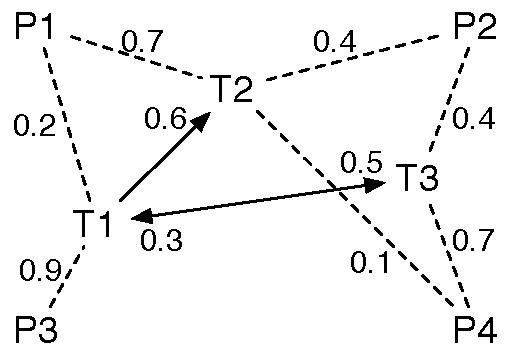
\includegraphics[width=.6\columnwidth]{figures/peopleTaskAssignment}
	\caption{An assignment/task-dependency network. 70\% of person P1's time is assigned to task T2, whereas T1 depends 60\% on task T2.}
	\label{fig:assignment}
\end{figure}

\begin{figure*}[t]
  \centering
  \subfigure[Coordination requirement derived from the given task assignment and task dependencies.]{
	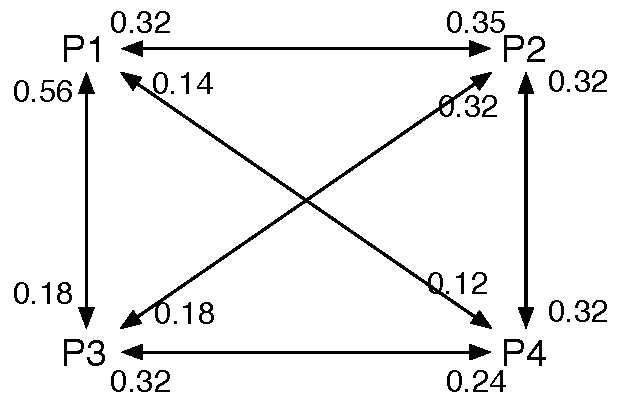
\includegraphics[width=0.65\columnwidth]{figures/coordRequirement}
     \label{subfig:coordRequ}
  }
  \subfigure[The coordination that happened.]{
    \includegraphics[width=0.65\columnwidth]{figures/actualCoord}
    \label{subfig:actualCoord}
  }
  \subfigure[The coordination that is lacking.]{
    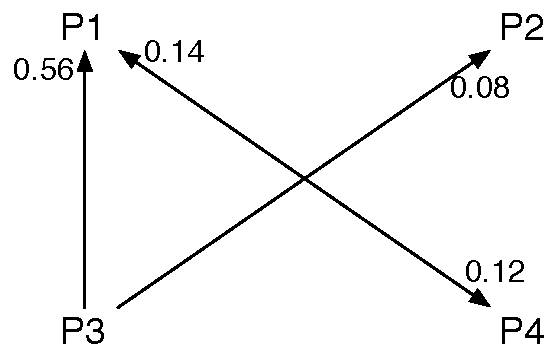
\includegraphics[width=0.65\columnwidth]{figures/coordLack}
    \label{subfig:coordLack}
  }
	\caption{Compare coordination requirements with actual coordination to find lacking coordination.}
	\label{fig:communication}
\end{figure*}


%------------------------------------------------------------------------- 
\Section{A Weighted Congruence Measurement}
\label{sec:measure}

In this section we introduce our measurement to weigh dependencies between tasks and between people and tasks.
This, combined with a weighted actual coordination, will result in a model that more accurately describes coordination.

\SubSection{Weighted Coordination Requirements}
\label{subsec:ourmeasure}

Our measurement applies weighted edges between 0 and 1 to the task assignment, task-dependency, and actual coordination matrices. Figure \ref{fig:assignment} shows an example of weights assigned to edges in a task assignment network. These weights are incorporated into the matrices required to calculate coordination requirements.

\begin{description}

\item[Weighted Task Assignment] matrix is a $m\times n$ matrix where $m$ is the number of selected people and $n$ denotes the number of selected tasks. 
Each entry in the matrix defines the strength of the connection between a person $i$ and a task $j$.

The weighted task assignment matrix may show how many hours one person is supposed to spend on a task. 
To break those values down to be between 0 and 1, they should be seen in the relation to the maximum work hours that person can spend.

One can also measure the expertise a person has about a task.
This would yield the amount of knowledge a person can share about a task.

\item[Weighted Task Dependency] matrix is a $n\times n$ matrix where $n$ denotes the number of selected tasks.
Each entry in the matrix describes the strength of the relation between two tasks.

The weighted task dependency matrix may show the ratio of dependencies a task has with another over the number of total dependencies that task has on others. 
For example, a task strongly coupled with another has a high task dependency.

\end{description}

To calculate the coordination requirements matrix, we follow the calculation proposed by Cataldo, et al.~\cite{cataldo2006:coordination_reqs}:
%
{\small$$\text{Task Assignment}\times\text{Task Dependency}\times\left(\text{Task Assignment}\right)^T$$}
%
%Given an actual coordination matrix, such as communication, we can calculate the congruence by dividing the number of actual coordination incidents that match the coordination requirement incidents over the total number of coordination requirement incidents.

This calculation will yield the coordination requirement matrix, which is a $m\times m$ people by people matrix (Figure \ref{subfig:coordRequ}).
The coordination requirement matrix tells you how strong the relations between people are supposed to be.


\SubSection{Weighted Congruence}

To derive the final congruence coefficient, the coordination requirements matrix needs to be compared to the actual observed coordination.
The comparison of the coordination requirements with the actual coordination follows three steps.

\begin{enumerate}
\item Create a people by people coordination matrix using our method (Figure \ref{subfig:coordRequ}).
\item Subtract the actual coordination matrix (Figure \ref{subfig:actualCoord}) from the coordination requirement matrix. This step differs from existing methods (e.g. \cite{cataldo2006:coordination_reqs,valetto2007}) that compute congruence with a ratio.
\item Set values that are less than zero to zero (Figure \ref{subfig:coordLack}).
\end{enumerate}

The resulting matrix illustrates areas that lack sufficient coordination to satisfy the coordination requirements. This matrix is  a \emph{lack-of-coordination matrix}  (Figure \ref{subfig:coordLack}) that identifies each gap along with its weight. The larger the value, the more severe the lack of coordination is.

To convert this lack-of-coordination matrix to a single socio-technical congruence measurement, sum the edge values and divide them by the sum of the edge values in the coordination requirements matrix. Then, subtract the result from 1 to get the congruence measurement.

%In the following we give an example on how to compute the coefficient.

%The social network is the network against which we compare to the coordination requirements network.
%These may be structural networks, geographical networks, and IRC-based networks, as in Cataldo~\cite{}, or they may be communication networks and awareness networks proposed in Damian~\cite{}.
%There are a number of other possible network types as well.
%Each of these can have weighted edges like the task assignment and task dependency networks.


%We can apply weights to different types of actual coordination matrices.
%Given a weighted coordination requirements matrix and a weighted actual coordination matrix, we can calculate different types of congruence.

\SubSection{Weighing Actual Coordination}

Different actual coordination measurements may be used for the congruence calculation. We present a few examples of techniques that can be used to weigh actual coordination matrices:

%Besides weighing the entries for the task assignment and task dependency matrices, we can also weigh the entries for the actual coordination. For example:


%\begin{description}
%\item[Task Assignment] 

%In Figure \ref{fig:assignment}, a connection between Person 1 (P1) and Task 1 (T1) is represented with an undirected edge of weight 0.2.

%\item[Task Dependency] 


%In Figure \ref{fig:assignment}, a connection between Task 1 (T1) and Task 2 (T2) is represented with a directed edge of weight 0.6.

%\end{description}

%Those are ways to weigh the different relationships between people and task or the inter relationships of task.
%The ways we described can reveal the need for better coordination or possible candidates for a knowledge transfer.



\begin{description}
\item[Communication] A social network such as a communication network can be weighed according to the amount of ongoing communication. Lets consider Alice and Bob that work on depended tasks:
\begin{enumerate}
	\item If Alice talks to Bob about his interdependent tasks, then for each task discussed the weight is increased by $a\cdot1/n$, where $a$ is the weight of the communication and $n$ is the number of Alice's tasks that depend on Bob's tasks.
	\item In case Alice discusses a task dependency very frequently with  Bob, then, given a three point scale ``occasionally/frequently/very frequently'', $a$ is set to 1. For another task that is only occasionally discussed, $a$ would be $0.\bar{3}$.
\end{enumerate}
In the end, if only two of Alice's tasks depend on Bob's tasks, the weight of Alice actual coordinating with Bob would be $1.0\cdot1/2+ 0.\bar{3}\cdot1/2= 0.6\bar{6}$.

\item[Distance] 
We can also measure the relationship between Alice and Bob by looking at different types of distance.
We can measure
\begin{itemize}
\item how far they are apart in terms of physical distance, like meters or kilometres,
\item the time difference between their time zones, and
\item the number of organizational units that part them.
\end{itemize}
These values are normalized to fit within 0 and 1. All three of those measures result in a symmetric matrix, meaning Alice will always have the same distance to Bob and vice versa.
\end{description}
	
After we weigh all entries within the task assignment, task dependency, and actual coordination matrix, we can compare the coordination requirements with the actual coordination using the method described in Section \ref{subsec:ourmeasure}.
%We discuss next the expected benefits from this weighted approach.

\SubSection{Illustration of Weighted Congruence}
In Figure~\ref{fig:assignment} we see two overlaid networks.
One connecting tasks with each other, the other connecting people with tasks.
In the task dependency network shows for example that task T$_1$ depends on task T$_2$ and the strength is denoted with $0.6$.
Whereas the allocation network in case of P$_1$ and T$_1$ that  person P$_1$ is allocated to work on task T$_1$ with dependency of strength $0.2$.
This dependency strength can for instance denote the percentage of time the person is supposed to dedicate to that task per day.

Figure~\ref{subfig:coordRequ} depicts the coordination requirements between people.
Looking at P$_1$ and P$_3$ shows that P$_3$ needs to coordinate quite a lot with P$_1$ but not the other way around.  
After subtracting the actual coordination (Figure~\ref{subfig:actualCoord}) from the coordination requirements yields a sparse network illustrated in Figure~\ref{subfig:coordLack}.
Only in four cases is coordination lacking.
The sum of the edge weights in Figure~\ref{subfig:coordRequ} is $3.37$.
Thus, the resulting congruence for this example is $1-[(0.56+0.14+0.08+0.12)/3.37] = 0.74$, whereas the traditional coefficient would have yielded a value of $0.9$, since there is only one coordination requirement not fulfilled (between P$_1$ and P$_3$).


%------------------------------------------------------------------------- 
\Section{The Benefit of Weighted Congruence}
\label{sec:benefit}

Using a weighted congruence model allows us to deal with situations that are not handled with regular congruence.
We can investigate relationships between people and the tasks in finer-grained detail, including situations where people are partially allocated to tasks. 
The measure can also provide a ranking of missing coordination: It suggests which lack-of-coordination gaps are most important to fill. Using the weighted congruence measure allows a person diagnosing the organization to utilize \emph{locality} and \emph{priority}.

\paragraph{Locality}
allows us to identify which area of a network has an issue to resolve.
Not only does this give us an overall measure of congruence, but now we can identify potential coordination problems in the network.
Although the original model does give us some limited locality in the sense of identifying congruence gaps, it is far more coarse grained.
For instance, using our weighted model, we can identify people working on two interdependent tasks who do not discuss both tasks.

\paragraph{Priority} 
ranks people pairs where more coordination might be needed by the computed lack of congruence.
Ranking is a considerable improvement over Cataldo's model since it allows us to only extract an unordered list of gaps. 
%This also covers gaps, but does not necessarily priorates gaps more.
Because filling congruence gaps can be risky~\cite{valetto2007:value,ehrlich2008:congruence_gaps}, a ranking can provides us with a better assessment of which gaps to fill first if at all.
\\ \ 
\indent By allowing better locality and priority, we believe that our weighted model of congruence provides a better way to study congruence and to diagnose issues.



%------------------------------------------------------------------------- 
\Section{Conclusions and Future Work}
\label{sec:conclusion}

We extend the socio-technical congruence measurement by proposing a model that involves weighted edges. 
By weighing each edge with a value between zero and one, we provide a method to weigh both gaps to decide which is more critical, as well as ongoing coordination that should be intensified.
This concept builds can identify properties of organization, such as locality to closer investigate the coordination network, and priority to see critical areas for improvement.

We are currently exploring additional schemes for weighting edges, and intend to conduct studies to determine their applications.
Our future plans include determining techniques that allow us to weigh the relationships between people and tasks, tasks and other tasks, and people and people.
We then intend to empirically investigate the weighing techniques that we suggest by applying them to various case studies.
By weighing people and tasks relationship, task interdependencies, and people interrelationships, we hope to more easily diagnose and resolve coordination issues.


%------------------------------------------------------------------------- 
\bibliographystyle{latex8}
\bibliography{stc09}

\end{document}

